\documentclass{article}
\bibliographystyle{plain}

\usepackage[utf8]{inputenc}
\usepackage[T1]{fontenc}
\usepackage[frenchb]{babel}
\usepackage{lmodern}
\usepackage{microtype}
\usepackage{graphicx}
\usepackage{pdfpages}

\title{%
  Rapport de Comité de Suivi de Thèse \\
  {\bf Analyse temporelle des systèmes temps-réel %multi-c{\oe}urs
    par vérification de modèles temporisés}}

\author{Armel Mangean}
\date{Juin 2016}

%% TODO: Ajouter des détails concernant mon avancement
%%  - dans la compréhension du sujet ;
%%  - mon analyse du sujet ;
%%  - la bibliographie.

\begin{document}
  \maketitle
  \tableofcontents

  \section*{Introduction}

  Ce rapport offre un aperçu du domaine dans lequel mon sujet de thèse se situe.
  %de son positionnement vis-à-vis de l'état de l'art dans ce domaine, du travail
  %de recherche réalisé dans cette direction à ce jour et des perpectives
  %dégagées pour le travail à venir.
  Il rend également compte brièvement de mes activités doctorales annexes au
  travail de recheche.

  \medskip

  Le travail réalisé à ce jour consiste en l'implémentation d'un outil de
  génération de modèles formels de programmes pour l'analyse temporelle par
  vérification. Le processus de génération est composé de deux étapes. La
  première réalise une reconstruction du graphe de flot de contrôle du
  programme à partir d'un fichier éxécutable. La seconde procède à la réduction
  du graphe de flot de contrôle par \textit{slicing}.

  \medskip

  Ce rapport est organisé comme suit. La section \ref{sec:biblio} expose l'état
  de l'art dans le domaine de la reconstruction de CFG. La section
  \ref{sec:work} détaille le travail d'implémentation d'un outil de
  reconstruction de CFG spécifiquement prévu pour l'analyse temporelle. La
  section \ref{sec:future} offre les perspectives envisagées pour développer une
  nouvelle approche d'analyse temporelle par vérification de modèles temporisés
  pour les plateformes multi-c{\oe}ur intégrant cet outil. La section
  \ref{sec:other} traite de mes activités doctorales annexes.

  \section{Travail réalisé}
\label{sec:work}
  \subsection{Reconstruction de CFG}
    \subsubsection{Définitions}
      \paragraph{Instructions et fichier exécutable}
      { Les instructions machine, ou simplement instructions, sont les
        opérations codées en langage machine qu'offre un processeur.

        Un fichier exécutable contient l'ensemble des instructions d'un
        programme écrit dans un langage de haut niveau (ou en assembleur) qui a
        été compilé (ou respectivement assemblé) pour une plateforme
        particulière. }
  
      \paragraph{Bloc de base et graphe de flot de contrôle}
      { Un bloc de base est une séquence d'instructions qui n'a qu'un point
        d'entrée, sa première instruction, et qu'un point de sortie, sa dernière
        instruction.

        Le graphe de flot de contrôle d'un programme est un graphe orienté dans
        lequel les n{\oe}uds représentent les blocs de base issus du programme
        et les transitions représentent les enchainements possibles entre les
        différents blocs de base lors de l'exécution du programme.
    
        De manière formelle, un CFG est un tuple $(V, E, i)$, où les n{\oe}uds
        $V$ correspondent aux blocs de bases, les transitions $E \subset V
        \times V$ sont les chemins du flots de contrôle et $i \in V$ représente
        le n{\oe}ud de départ, c'est à dire le n{\oe}ud qui n'a pas de
        transition entrante. }

    \subsubsection{Méthodes de reconstruction}

      % Utilisation d'un analyseur sémantique de fichiers exécutables pour la
      % reconstruction de CFG.

      Le fichier exécutable à analyser est en amont soumis à une analyse
      sémantique réalisée par l'outil \textsc{HARMLESS}~\cite{KBB12}. Cette
      analyse séquentielle des instructions du fichier exécutable produit un
      fichier de données textuelles associant à chaque instruction un ensemble
      d'informations la caractérisant. Parmi ces informations on peut citer par
      exemple : l'adresse mémoire de l'instruction, une representation textuelle
      de l'instruction issue de son désassemblage, ou encore les registres
      utilisés en lecture et en écriture par l'instruciton. Ce fichier de
      données est l'unique entrée de l'outil décrit ici.

      \medskip

      Cet outil\footnote{\texttt{https://github.com/LiberH/tool}} est écrit en
      Haskell~\cite{Mar10}. Il réalise de manière préliminaire une analyse
      syntaxique du ficher d'entrée pour en manipuler le contenu via une
      strucutre de données appropriée. Cette structure représente la liste
      ordonnée des instructions du programme.
      
      \begin{figure}
        \centering
        \includegraphics[scale=0.3]{recons1.eps}
        \caption{Processus de reconstruction de blocs de base}
        \label{fig:recons1}
      \end{figure}

      \paragraph{Reconstruction des blocs de base}
      { La prémière étape nécessaire à la reconstruction du CFG consite en la
        reconstitution des blocs de base du programme.

        Pour ce faire, il est tout d'abord nécessaire d'identifier les points
        d'entrée de blocs de base. Une instruction est une entrée de bloc de base
        si elle se trouve être :
        \begin{itemize}
          \item le point d'entrée du programme ;
          \item une cible de saut ;
          \item immédiatement après une instruction de saut ;
          \item la première instruction du fichier exécutable.
        \end{itemize}

        Les blocs de base sont construits en parcourant séquentiellement la
        liste ordonnée des instructions du programme et par accumulation des
        instructions se trouvant entre un point d'entrée de bloc de base inclus
        jusqu'au suivant exclus. La figure \ref{fig:recons1} donne un exemple
        d'un telle reconstruction. }

      \begin{figure}
        \centering
        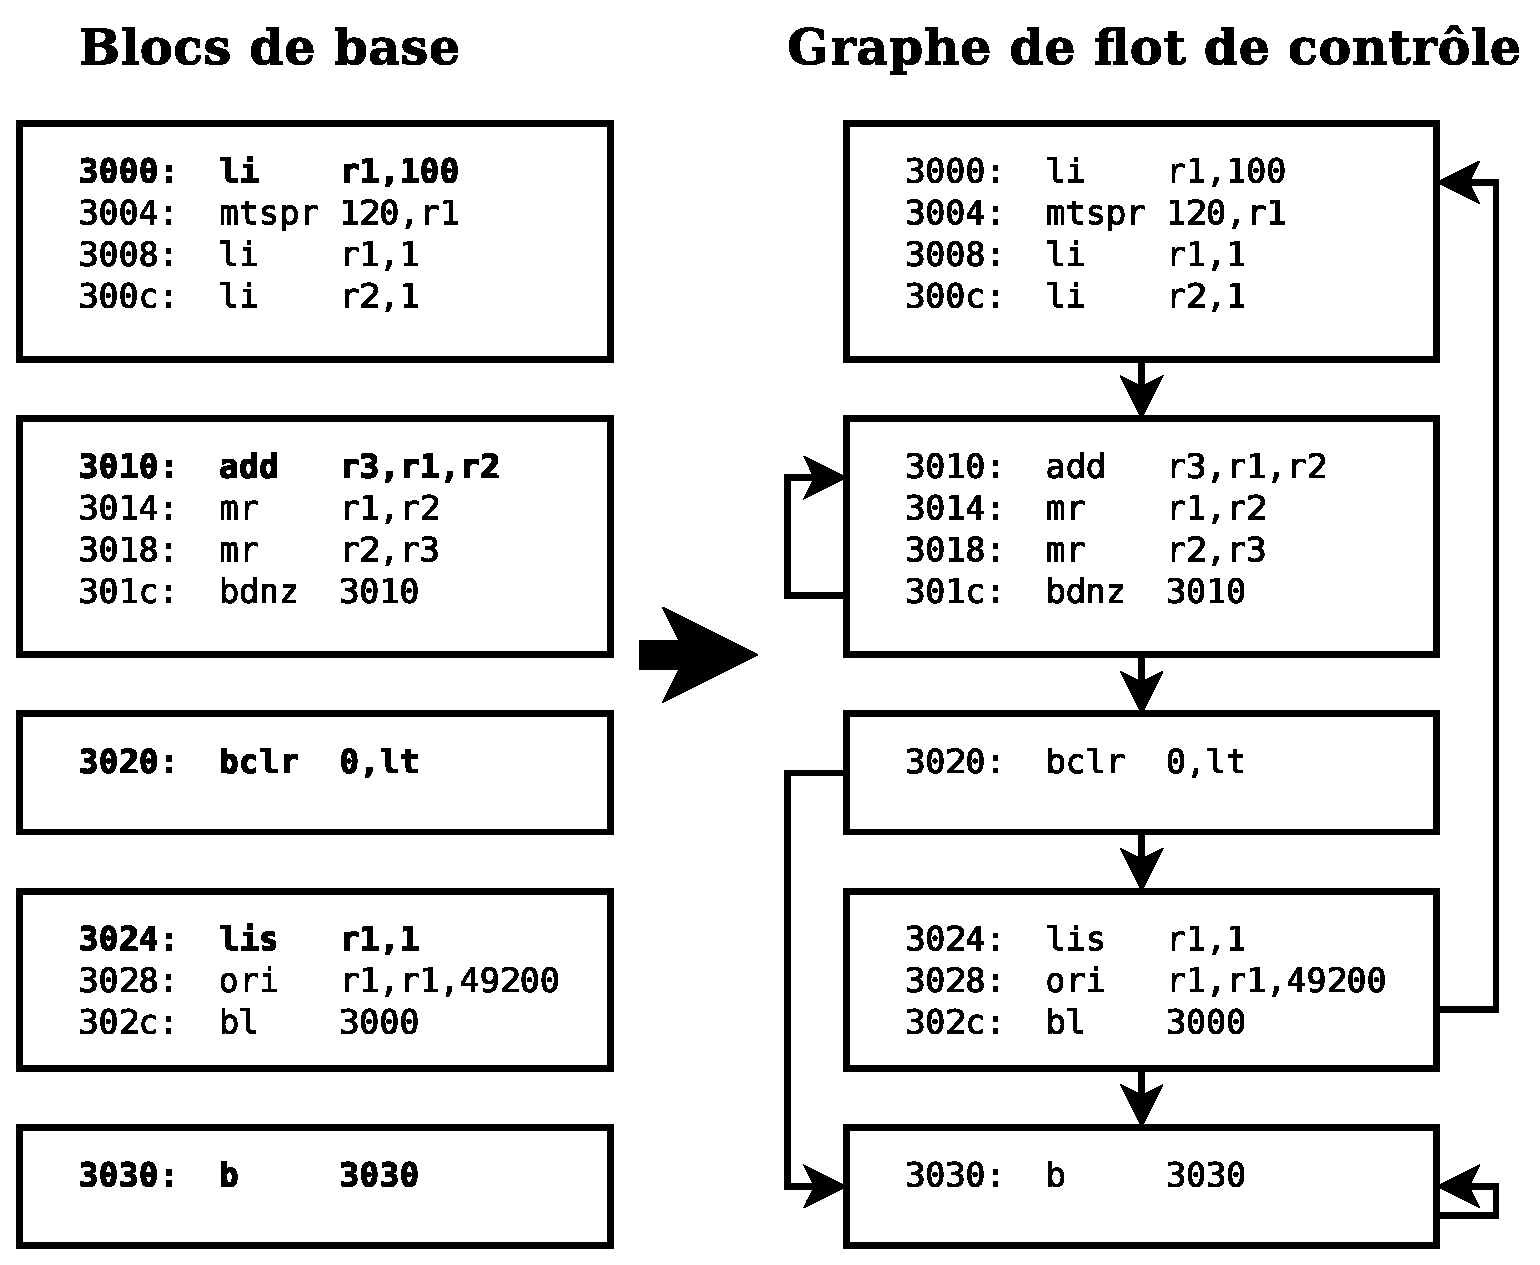
\includegraphics[scale=0.3]{recons2.eps}
        \caption{Processus de reconstruction d'un CFG}
        \label{fig:recons2}
      \end{figure}

      \paragraph{Reconstruction de CFG}
      { % Utilisation d'une bibliothèque d'analyse et de transformation de CFG
        % pour le slicing de CFG.

        Afin de procéder à la reconstruction du CFG en elle-même l'outil fait
        usage de \textsc{Hoopl}, une bibliothèque de manipulation de CFG en
        Haskell~\cite{RDP10}. Cette bibliothèque permet de définir simplement
        des analyses de flots de données ainsi que des transformations sur les
        CFG manipulés.

        \medskip
        
        Il est tout d'abord nécessaire d'identifier les n{\oe}uds. C'est une
        tâche triviale vis-à-vis de la définition d'un CFG. Il faut également
        identifier le n{\oe}ud de départ. C'est le n{\oe}ud correspondant au
        bloc de base issu du point d'entrée du programme.

        Il faut ensuite contruire les transitions. Elles sont obtenues
        itérativement en associant à chaque bloc de base les cibles possibles de
        son point de sortie. La figure \ref{fig:recons2} donne un exemple d'un
        telle reconstruction.

        Cette tâche est difficile dans le cas de sauts indirects. Lorsqu'il est
        impossible de déterminer les cibles possibles du point de sortie d'un
        bloc de base il est fait usage d'un n{\oe}ud \textit{inconnu}. Ces
        cibles seront par la suite déterminées par le \textit{slicing} du CFG. }
        

  %% TODO:
  %\subsection{Slicing de CFG}

  %% Cet article décrit le travail d'implémentation d'un outil de génération de
%% modèles de programmes. Cette implémentation fait partie d'un travail de
%% développement d'une approche d'analyse temporelle des systèmes embarqués
%% temps-réel par vérification de modèles temporisés.
%% 
%% Pour ce faire, les modèles produits sont générés sous forme d'automates finis
%% représentant les CFG des programmes considérés. Les modèles produits sont issus
%% de reconstructions de CFG à partir de fichiers exécutables. Leur taille est
%% limitée en nombre de n{\oe}ud par \textit{program slicing} des CFG.

%% Les microprocesseurs multi-c{\oe}urs sont de plus en plus employés dans l'embarqué
%% temps-réel à des fins de performances et de baisse de consommation d'énérgie.
%% 
%% À la différence des approches existantes d'analyse temporelle par vérification
%% de modèles, l'approche en développement se veut adaptée aux plateformes
%% matérielles multi-c{\oe}urs.

\section{Perspectives}
\label{sec:future}

% Déjà dit en intro
  %La méthode de génération automatique de modèles de programmes qui a été
  %décrite ci-dessus fait partie d'un travail de développement d'une approche
  %d'analyse temporelle des systèmes embarqués temps-réel par vérification de
  %modèle temporisé de ce point de vue similaire à différentes méthodes
  %existantes \cite{CB13, DOT10}.

  \subsection{Modélisation d'une plateforme multi-c{\oe}ur}

    %% % Inéviatbilité de l'utilisation de plateformes multi-c{\oe}urs dans le futur.
    %% 
    %% L'utilisation futur de plateformes multi-c{\oe}urs dans les systèmes
    %% temps-réel semble inévitable et ce à des fins de performances et de
    %% baisse de consommation d'énérgie.

    % Problèmatique des plateformes multi-c{\oe}urs pour l'analyse temporelle.

    Il est largement considéré aujourd'hui que les multi-c{\oe}urs
    seront massivement employés dans le futur de l'embarqué temps-réel à des
    fins de performances et de baisse de consomation d'énérgie. Le problème qui
    se pose est que de telles plateformes ne fournissent pas forcemment de
    garanties sur les propriétés temps-réel des logiciels s'exécutant dessus.

    Les bus de données partagés font partie des équipements les plus critiques
    de ce point de vue du fait des possibles conflits d'accés entre les
    différents c{\oe}urs. De part leur complexité de fonctionnement, on constate
    qu'ils abaissent significativement la precision des calculs de WCET des
    plateformes multi-c{\oe}urs.

    Les temps d'accès à des données en mémoire sont très variables selon qu'ils
    sont réalisés vers la mémoire centrale ou la mémoire cache. Il est donc
    nécessaire de modéliser fidélement la mémoire cache sans quoi les calculs de
    WCET ne peuvent être précis.

    %% % Incompatibilité avec les analyses temporelles actuelles.
    %% 
    %% Cependant, les analyses temporelles actuelles se limitent le plus souvent au
    %% calcul des pires temps d'exécution des tâches en isolation.
    %%
    %% Il nous parrait nécessaire d'étendre l'analyse temporelle des systèmes
    %% embarqués temps-réel pour tenir compte des comportements spécifiques qui
    %% peuvent advenir lors de l'exécution parellèle de plusieurs tâches.

    \vspace{1em}

    % Perspectives associées.

    L'une des ambitions de ce travail est d'étudier l'intérêt des méthodes
    d'analyse temporelle basées sur la vérification de modèles temporisés pour
    les plateformes matérielles multi-c{\oe}urs. Pour ce faire, un modèle
    temporisé d'une plateforme multi-c{\oe}ur PowerPC sera réalisé.  L'analyse
    temporelle portera sur les systèmes obtenus par produit synchronisé de ce
    modèle et des modèles logiciels engendrés par la méthode décrite ci-dessus.

  \subsection{Spécialisation de la vérification}

    % Problèmatique des plateformes multi-c{\oe}urs pour la vérification de modèle.

    La modélisation d'une plateforme matérielle complexe implique un nombre de
    localités et d'horloges important dans le modèle. De fait, malgrès la
    réduction du modèle logiciel grâce à la technique qui a été décrite ici, la
    vérification risque de ne pas aboutir
    soit par manque d'espace mémoire, soit du fait d'un temps de traitement trop
    important dû à l'explosion de la taille de l'espace d'état à traiter.

    \vspace{1em}

    % Perspectives associés.

    Pour pallier ce problème, les algorithmes et structures de données utilisés
    pour la vérification seront spécialisés. Cette spécialisation exploitera
    des propriétés de monotonie pour couper rapidement des branches lors de
    l'exploration de l'espace d'état.

    Ces résultats seront comparés rigouresement aux temps d'exécution mesurés sur une
    plateforme physique PowerPC multi-c{\oe}urs dont le modèle aura été réalise.
    Parmi les programmes dont les WCET seront calculé on retrouvera les
    programmes du banc d'essai de Mälardalen \cite{GBA10} dont les WCET réels
    sont connus.  
    %La méthode de génération automatique de modèles de programmes
    %qui a été décrite ci-dessus fait partie d'un travail de developpement d'une
    %approche d'analyse temporelle des systèmes embarqués temps-réel par
    %vérification de modèle temporisé de ce point de vue similaire à différentes
    %méthodes existantes \cite{CB13, DOT10}.

  \section{Activités annexes}
\label{sec:other}
  \subsection{Enseignement}

    Durant l'année universitaire courante j'ai pu effectuer un peu plus de 77
    heures d'encadrement en vacation auprés d'étudiants en première et deuxième
    année de DUT Informatique -- voir ci-dessous pour le détail des
    enseignements dispensés. Cela représente près de 64 heures équivalent TD, le
    nombre maximal d'heures d'encadrement autorisées par an. Soit au total, en
    les cumulant aux heures d'encadrement effectuées l’année universitaire
    précédente, 114 heures de d'encadrement en vacation.
    
    \paragraph{<< Administration Système et Réseau >>}
    { \begin{itemize}
        \item Du 25 Janvier au 21 Mars ;
        \item 14 TD de 1h20 chacun ;
        \item Cours de DUT Informatique deuxième année ;
        \item Déploiement et sécurité des infrastructures réseaux. 
      \end{itemize} }

    \paragraph{<< Architecture et Programmation >>}
    { \begin{itemize}
        \item Du 29 Janvier au 25 Mars ;
        \item 5 TD et 17 TP de 1h20 chacun ;
        \item Cours de DUT Informatique première année ;
        \item Jeu d'instruction IA-32 et \emph{reverse engineering}.
      \end{itemize} }

    \paragraph{<< Architecture des Réseaux >>}
    { \begin{itemize}
        \item Du 28 Avril au 16 Juin ;
        \item 7 TD et 14 TP de 1h20 chacun ;
        \item Cours de DUT Informatique première année ;
        \item Modèle OSI et pile TCP/IP, fonctionnement des couches réseaux
          basses.
      \end{itemize} }

  \subsection{Formation doctorale}

    Au cour des 3 ans de doctorat, un minimum 100 heures de formation doivent
    être validées. Ces heures doivent être réparties équitablement entre
    formation professionelle et formation scientifique.
    
    Durant l'année universitaire courante j'ai pu valider 61 heures de formation
    doctorales dont 36 heures de formation professionnelle et 25 heures de
    formation scientifique -- voir ci-dessous pour le détail des formations
    suivies. Soit au total, en les cumulant aux heures de formations validées
    l'année universitaire précédente, 53 heures de formation professionnelle et
    40 heures de formation scientifique.

    Au cour de l'année universitaire à venir, je devrais suivre une formation
    scientifique de 10 heures ou plus afin de remplir le contrat des 100 heures
    de formation minimum.
  
    \paragraph{<< École d'été MOVEP 2014 >>}
    { \begin{itemize}
        \item À Nantes, du 7 au 11 juillet 2014 ;
        \item Validant 15 heures de formation scientifique ;
        \item Enseignements pour les jeunes chercheurs sur divers aspects de
          modélisation et vérification des applications.
      \end{itemize} }

    \paragraph{<< Journée des doctorants >>}
    { \begin{itemize}
        \item À Nantes, le 21 avril 2016 ;
        \item Validant 10 heures de formation scientifique ;
        \item Rencontre des doctorants de l'école doctorale STIM inscrits en
          deuxième année.
      \end{itemize} }

    \paragraph{<< Regard Neuf : initiation à la pratique du conseil >>}
    { \begin{itemize}
        \item À Nantes, les 20 novembre, 17 et 18 décembre 2015 ;
        \item Validant 18 heures de formation professionnelle ;
        \item Initiation au conseil en entreprise par équipe pluridisciplinaires
          de huit doctorants sur des problématiques réelles en partenariats avec
          des entreprises locales.
      \end{itemize} }

    \paragraph{<< Research : Methodology and strategy >>}
    { \begin{itemize}
        \item À Nantes, les 10, 12, 18, 24 et 25 novembre 2015 ;
        \item Validant 18 heures de formation professionnelle ;
        \item Information et discussions sur de nombreux aspects de
          la Recherche (en anglais).
      \end{itemize} }
  


  \bibliography{refs.bib}

  \appendix\vfill
  
  %% \section{Poster accépté à SoC -- SiP'16}
  %% \label{sec:socsip16}
  %% \emph{(cf. page suivante)}
  %% \includepdf[page=1-,frame, scale=.9]{img/socsip16.pdf}

  \section*{\huge Annexes}
  \section{Article soumis à WCET'16}
  \label{sec:wcet16}
  \emph{(cf. page suivante)}\vfill
  \includepdf[page=1-,frame, scale=.9]{img/wcet16.pdf}

\end{document}
